\documentclass[conference]{IEEEtran}
\IEEEoverridecommandlockouts
% The preceding line is only needed to identify funding in the first footnote. If that is unneeded, please comment it out.
\usepackage{cite}
\usepackage{amsmath,amssymb,amsfonts}
\usepackage{algorithmic}
\usepackage{graphicx}
\usepackage{textcomp}
\usepackage{xcolor}
\usepackage{booktabs}
\usepackage{multirow}
\usepackage{tikz}
\usetikzlibrary{positioning,arrows.meta,fit,backgrounds}
\def\BibTeX{{\rm B\kern-.05em{\sc i\kern-.025em b}\kern-.08em
    T\kern-.1667em\lower.7ex\hbox{E}\kern-.125emX}}
\graphicspath{{figures/}}
\newtheorem{proposition}{Proposition}

\begin{document}

\title{CertiVOI: Certified Triage of Repeat Laboratory Tests by Their Chance of Changing the Clinical Action}

\author{\IEEEauthorblockN{1\textsuperscript{st} Given Name Surname}
\IEEEauthorblockA{\textit{dept. name of organization} \\
\textit{name of organization}\\
City, Country \\
email address or ORCID}
\and
\IEEEauthorblockN{2\textsuperscript{nd} Given Name Surname}
\IEEEauthorblockA{\textit{dept. name of organization} \\
\textit{name of organization}\\
City, Country \\
email address or ORCID}
}

\maketitle

\begin{abstract}
A considerable fraction of inpatient blood tests are repeats whose results leave the plan of care unchanged. Existing approaches flag such tests by forecasting whether the next value will be normal or close to the previous one, yet neither property tells whether the result would alter a decision, and none of these approaches limits how many consequential results a reduction policy would suppress. This paper presents CertiVOI, which estimates, before a repeat test is drawn, the probability that the new value lands in a different guideline-defined action category from the most recent one. A quantile gradient-boosting model yields a predictive distribution for the new value, and the probability mass lying outside the current category serves as the score; under a 0--1 regret this score coincides with the single-step value of information. Conformal risk control then fixes a threshold so that the expected fraction of missed action changes does not exceed a user-chosen level $\alpha$. Two extensions target deployment: certification at the level of the blood draw, because analytes sharing a tube are skipped together, and an online threshold update that learns from a small random audit of the tests it suppresses. On 285,659 repeat tests from 40,336 ICU patients treated at two hospitals, the certified tier contained 38--74\% of hemoglobin, potassium and creatinine tests at $\alpha=1\%$. A hemoglobin threshold transferred without adjustment to the second hospital missed 16.8\% of tests at a nominal $\alpha=5\%$; the audited update restored the rate to 5.0\%.
\end{abstract}

\begin{IEEEkeywords}
laboratory test utilization, value of information, conformal risk control, quantile regression, distribution shift, clinical decision support
\end{IEEEkeywords}

\section{Introduction}
Routine laboratory monitoring is one of the most frequent activities in hospital care. Electrolytes, blood counts and renal markers are commonly redrawn every morning, and in intensive care several times a day. Each draw consumes staff time and reagents, and for critically ill patients the accumulated phlebotomy volume contributes to iatrogenic anemia. Clinicians generally accept that part of this testing is redundant; the difficulty lies in recognizing, in advance, which specific test can be omitted without consequence.

Prior predictive work has framed the problem statistically, asking whether the coming result will fall within the reference range \cite{xu2019lowyield} or remain close to its predecessor \cite{aikens2023yield}, and recurrent networks have been trained to recommend reductions on the same basis \cite{yu2020deep,li2022external,huang2023confidence}. Decision analysis poses a sharper question: a test carries value only when at least one of its plausible results would lead to a different action \cite{howard1966,pauker1980}. The DECIDE-Lab framework recently applied this principle to laboratory testing \cite{allenbrand2026decidelab}, although with priors and utilities specified by hand rather than estimated from records. The distinction matters in practice. A potassium of 5.0~mEq/L is normal, yet in a patient receiving replacement for hypokalemia it is precisely the value that ends the therapy. Conversely, a fourth consecutive hemoglobin of 7.8~g/dL is abnormal but, on its own, would not prompt a transfusion.

A further obstacle is assurance. In a pre-implementation study of an EHR-embedded reduction tool, clinicians asked for near certainty before any test would be discouraged \cite{rabbani2023targeting}. Published models, however, report discrimination rather than an explicit limit on the number of consequential results a reduction rule would hide.

The contributions of this work are as follows:
\begin{itemize}
\item An action-anchored target for repeat testing, together with evidence from two datasets that normality and stability labels frequently disagree with it.
\item A score derived from a quantile forecaster, linked formally to value of information, and a low-value tier certified by conformal risk control (CRC) \cite{angelopoulos2024crc}.
\item To our knowledge, the first certification of complete blood draws, accompanied by a demonstration that analyte-level guarantees do not compose.
\item An audit-driven online threshold with a long-run bound that holds without exchangeability, evaluated on a hospital excluded from training.
\end{itemize}

\section{Related Work}
\textit{Low-yield testing.} Xu et al. predicted normal results for common inpatient assays \cite{xu2019lowyield}; Aikens et al. estimated the probability that a repeat value would match the preceding one \cite{aikens2023yield}. Yu et al. and subsequent studies used recurrent models on ICU records and added a confidence filter to their reduction recommendations \cite{yu2020deep,li2022external,huang2023confidence}. All of these optimize a surrogate of action change, and none bounds the rate of missed results that matter.

\textit{Sequential acquisition.} Reinforcement learning can learn ordering policies across many tests \cite{yu2023drl}, but such policies require extensive data, resist inspection and lack finite-sample guarantees. We address the narrower per-test decision.

\textit{Conformal control.} CRC chooses a threshold that keeps the expectation of a monotone loss below $\alpha$ \cite{angelopoulos2024crc}, Learn-then-Test (LTT) provides high-probability control \cite{angelopoulos2021ltt}, and Mondrian schemes calibrate within strata \cite{vovk2005alrw}. Under temporal drift, adaptive conformal inference \cite{gibbs2021aci} and rolling risk control \cite{feldman2023online} revise the threshold after every observation, which presumes that each label is revealed. When a test is skipped, its label is never produced, a situation closer to partial-feedback conformal prediction \cite{ge2024semibandit}. Hierarchical data with repeated measurements per subject have been studied for prediction sets \cite{dunn2023hierarchical}.

\section{Method}
\begin{figure}[t]\centering
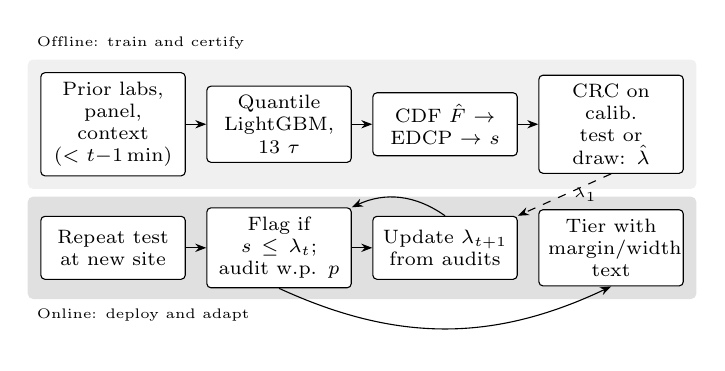
\begin{tikzpicture}[node distance=3mm and 2.6mm, every node/.style={font=\scriptsize,align=center},
  box/.style={draw,rounded corners=1.5pt,minimum height=8mm,text width=16mm,fill=white},
  >={Stealth[length=1.4mm]}]
\node[box] (a) {Prior labs, panel,\\context ($<t{-}1$\,min)};
\node[box,right=of a] (b) {Quantile\\LightGBM, 13 $\tau$};
\node[box,right=of b] (c) {CDF $\hat F$ $\rightarrow$\\EDCP $\rightarrow$ $s$};
\node[box,right=of c] (d) {CRC on calib.\\test or draw: $\hat\lambda$};
\node[box,below=5mm of a] (e) {Repeat test\\at new site};
\node[box,right=of e] (f) {Flag if $s\le\lambda_t$;\\audit w.p. $p$};
\node[box,right=of f] (g) {Update $\lambda_{t+1}$\\from audits};
\node[box,right=of g] (h) {Tier with\\margin/width text};
\draw[->] (a)--(b); \draw[->] (b)--(c); \draw[->] (c)--(d);
\draw[->] (e)--(f); \draw[->] (f)--(g); \draw[->] (f.south) to[bend right=25] (h.south);
\draw[->] (g.north) to[bend right=30] (f.north east);
\draw[->,dashed] (d.south) -- node[right,font=\tiny]{$\lambda_1$} (g.north east);
\begin{scope}[on background layer]
\node[fill=black!6,rounded corners=2pt,fit=(a)(d),inner sep=1.6mm,label={[font=\tiny,anchor=south west]north west:Offline: train and certify}] {};
\node[fill=black!12,rounded corners=2pt,fit=(e)(h),inner sep=1.6mm,label={[font=\tiny,anchor=north west]south west:Online: deploy and adapt}] {};
\end{scope}
\end{tikzpicture}
\caption{Overview of CertiVOI. The offline stage forecasts the new value and certifies a threshold on held-out patients; the online stage adapts the threshold at a new site from audited tests.}\label{fig:pipeline}
\end{figure}

\subsection{Action-anchored label}
Let $e$ index a resulted measurement $y_e$ of laboratory $L$ taken at time $t_e$ during an admission that already holds a value of $L$ within the preceding 72~h. Predictors are restricted to information recorded before $t_e-1$~min. An action map $A_L$ assigns each value to a management category. We adopt simplified guideline cut-offs: hemoglobin $<7$, $7$--$8$ and $\ge 8$~g/dL \cite{carson2016aabb}; potassium $<3.5$, $3.5$--$5.5$ and $>5.5$~mEq/L; platelets $<10$, $10$--$50$ and $\ge 50\times10^3/\mu$L \cite{kaufman2015platelet}. For creatinine the category is the KDIGO stage \cite{kdigo2012}, determined by a rise of at least 0.3~mg/dL above the 48-h minimum, by ratios of 1.5, 2 and 3 to the 7-day minimum, or by an absolute value of 4.0~mg/dL. Writing $a^0_e$ for the category of the most recent prior value $y^{\text{last}}_e$, the target is
\begin{equation}
D_e=\mathbb{1}\big[A_L(y_e)\neq a^0_e\big].
\label{eq:label}
\end{equation}
For comparison, the proxy $N_e$ marks a value inside the reference range and $S_e$ marks an absolute change no larger than 0.5~g/dL, 0.3~mEq/L, 0.2~mg/dL or $20\times10^3/\mu$L.

\subsection{Distributional forecast and EDCP}
For every laboratory, LightGBM \cite{ke2017lightgbm} is fitted with the pinball loss \cite{koenker1978} at thirteen levels $\tau\in\{0.02,\dots,0.98\}$ to the change $y_e-y^{\text{last}}_e$. The 53--55 predictors summarize the analyte's own trajectory (recent values, 48-h slope, counts and elapsed time), companion analytes from the same panels, and context such as age, sex and time since admission. After monotone rearrangement \cite{chernozhukov2010}, the quantiles define a piecewise-linear distribution function $\hat F$. With $[l_a,u_a)$ denoting the interval of category $a$, the expected decision-change probability (EDCP) is
\begin{equation}
\mathrm{EDCP}(x_e)=1-\big[\hat F(u_{a^0_e}\mid x_e)-\hat F(l_{a^0_e}\mid x_e)\big].
\label{eq:edcp}
\end{equation}
For creatinine the interval limits are recomputed for each event from its own baselines. EDCP is mapped through isotonic regression fitted on validation patients to give the score $s_e$.

\begin{proposition}
Assume that the test reveals the category $c$, that the clinician then acts on $c$, that without the test the default $a^0$ is retained, and that the regret is $r(a,c)=\mathbb{1}[a\neq c]$. Then the value of information of the test equals $\Pr(c\neq a^0\mid x)$, the quantity estimated by \eqref{eq:edcp}.
\end{proposition}
\begin{IEEEproof}
The expected regret avoided is $\mathbb{E}_c[r(a^0,c)-r(c,c)]=\mathbb{E}_c[\mathbb{1}(c\neq a^0)]$.
\end{IEEEproof}

\subsection{Certified low-value tier}
A test is labelled low value when $s_e\le\lambda$, and suppressing it incurs the loss $\ell_e(\lambda)=D_e\mathbb{1}[s_e\le\lambda]$, which is non-decreasing in $\lambda$. Given $n$ calibration events drawn from patients unseen during training, CRC selects
\begin{equation}
\hat\lambda=\max\Big\{\lambda:\ \textstyle\sum_{i=1}^{n}\ell_i(\lambda)+1\le\alpha(n+1)\Big\},
\label{eq:crc}
\end{equation}
which ensures $\mathbb{E}[\ell_{\text{new}}(\hat\lambda)]\le\alpha$ whenever calibration and future events are exchangeable \cite{angelopoulos2024crc}. Put differently, action changes concealed by the tier make up at most a fraction $\alpha$ of all repeat tests. LTT with exact binomial p-values is run alongside; it bounds the miss rate among flagged tests by $\beta$ with probability $1-\delta$ \cite{angelopoulos2021ltt}. Scores above a validation cut-off with precision 0.5 form a high-value tier, and the remainder are labelled potentially useful.

Because repeat tests of one patient are dependent whereas patients are exchangeable by design of the split, we also apply \eqref{eq:crc} at the patient level, replacing $\ell_i$ by the patient average $L_i(\lambda)=m_i^{-1}\sum_{e\in i}\ell_e(\lambda)$. The resulting guarantee concerns the expected share of missed changes within a new patient.

\subsection{Draw-level certification}
Hemoglobin and platelets are measured from one CBC tube, and potassium and creatinine from one chemistry tube. A draw may be omitted only when all of its analytes are low value, and it conceals a change whenever any analyte changes category. If each analyte $j$ of panel $P$ is certified separately at level $\alpha$ and the draw is omitted when all are flagged, a concealed change implies at least one flagged analyte with $D_j=1$; the union bound then gives only $|P|\alpha$. Bonferroni correction ($\alpha/|P|$ per analyte) restores validity at the cost of efficiency. We instead define $D_P=\max_j D_j$ and the draw score $s_P=1-\prod_j(1-s_j)$, and apply \eqref{eq:crc} to draws. The guarantee holds for any choice of $s_P$; the choice affects only the number of draws avoided.

\subsection{Online control with audited feedback}
The guarantee in \eqref{eq:crc} relies on similarity between calibration and deployment. At a new site the threshold should adapt, but a suppressed test yields no result from which to learn. We therefore perform each flagged test anyway with probability $p$, independently of all else. Let $u_t$ be the rank of $s_t$ among calibration scores, $f_t=\mathbb{1}[u_t\le\lambda_t]$ the flag, $A_t$ the audit indicator and $\hat\ell_t=D_tf_tA_t/p$, which requires $D_t$ only for tests actually run. The threshold, initialized at the rank of $\hat\lambda$, evolves as
\begin{equation}
\lambda_{t+1}=\min\big\{\lambda_t+\eta(\alpha-\hat\ell_t),\,1\big\}.
\label{eq:online}
\end{equation}

\begin{proposition}
For any sequence of scores and outcomes, \eqref{eq:online} satisfies $T^{-1}\sum_{t\le T}\hat\ell_t\le\alpha+\{\lambda_1+\eta(p^{-1}-\alpha)\}/(\eta T)$.
\end{proposition}
\begin{IEEEproof}
Truncation at one can only decrease $\lambda$, so $\lambda_{T+1}-\lambda_1\le\eta\sum_t(\alpha-\hat\ell_t)$. If $\lambda_t<0$ no test is flagged and $\lambda$ increases, while from $\lambda_t\ge0$ a single step reduces it by at most $\eta(p^{-1}-\alpha)$. Hence $\lambda_t\ge-\eta(p^{-1}-\alpha)$ for every $t$, and rearrangement yields the claim.
\end{IEEEproof}

Since audits are independent, $\mathbb{E}[\hat\ell_t\mid\text{history},s_t,D_t]=D_tf_t$; the realized and estimated miss rates therefore differ by an average of bounded martingale increments that vanishes at rate $O(p^{-1}T^{-1/2})$. The long-run miss rate is thus at most $\alpha$ asymptotically, whatever the drift. Audited tests are still drawn, so the effective reduction equals the share of tests that are flagged and not audited.

\subsection{Explanation}
For each prediction we report the median forecast $\hat y$, its signed margin $m$ to the nearest boundary of the current category, and the 80\% interval width $w=\hat q_{0.9}-\hat q_{0.1}$. A test is uninformative either because $\hat y$ lies far from a threshold or because the forecast is tight, and $\rho=m/w$ combines the two. Interventional TreeSHAP \cite{lundberg2017unified,lundberg2020trees} applied to the median model attributes the margin, and the difference between attributions of the $\tau=0.9$ and $\tau=0.1$ models attributes the width. The leading attributions are rendered as a short structured sentence.

\section{Experimental Setup}
\textit{Data.} The primary cohort is the public training set of the PhysioNet/Computing in Cardiology Challenge 2019 \cite{reyna2020sepsis,goldberger2000physionet}, comprising 40,336 adult ICU stays from two hospital systems (A: 20,336; B: 20,000) recorded at hourly resolution. The sepsis label was not used. The cohort contained 74,681 repeat hemoglobin, 102,820 potassium, 54,921 creatinine and 53,237 platelet tests. The eICU demonstration database \cite{pollard2018eicu} (1,836 patients, 186 hospitals, minute-level timestamps) served as a replication set.

\textit{Protocol.} Patients were allocated at random to training, validation, calibration and test sets (60/10/15/15\%; 18,127, 3,022, 4,532 and 4,532 patients with an eligible test). For external evaluation, models and thresholds were built on hospital A only and applied to the 13,867 eligible hospital B patients. CRC validity was assessed over 100 random re-partitions of held-out patients into calibration and test halves, and confidence intervals were obtained from 1,000 patient-level bootstrap samples.

\textit{Comparators.} B1 is a rule that skips a test when the last value requires no action, the last two values differ by less than the stability margin and fewer than 24~h have elapsed. B2 and B3 are LightGBM classifiers of normality and stability. B4 (logistic regression) and B5 (LightGBM) are trained on $D$ directly. Every score was additionally passed through the same CRC step. The online update used $\eta=0.002$ and $p\in\{0.2,0.1\}$, averaged over five random seeds; SHAP values were computed for 5,000 test events per laboratory.

% source: results\challenge2019/cohort/flow.csv, results\challenge2019/E1/table2_labels.csv, results\eicu_demo/E1/table2_labels.csv
\begin{table}[t]\centering\footnotesize
\caption{Repeat tests and how often action changes look ``normal'' or ``stable''.}
\label{tab:cohort}\setlength{\tabcolsep}{3pt}
\begin{tabular}{lrrrrrr}\toprule
 & & & & \multicolumn{2}{c}{Share of $D{=}1$ (\%)} & eICU \\ \cmidrule(lr){5-6}
Lab & Tests & Patients & $D{=}1$ (\%) & normal & stable & normal \\ \midrule
Hemoglobin & 74,681 & 26,771 & 10.3 & 0.9 & 15.5 & 1.2 \\
Potassium & 102,820 & 28,909 & 14.4 & 73.8 & 19.9 & 75.1 \\
Creatinine & 54,921 & 26,157 & 12.4 & 24.4 & 23.8 & 21.0 \\
Platelets & 53,237 & 25,408 & 2.1 & 1.7 & 50.9 & 1.2 \\
\bottomrule\end{tabular}\end{table}


\section{Results}
\subsection{Disagreement between action and proxy labels}
Table~\ref{tab:cohort} reports the prevalence of action changes and the share that each proxy would have classed as uninformative. Potassium shows the starkest mismatch: 73.8\% of action-changing results were within the reference range, a figure reproduced almost exactly on eICU (75.1\%). In 70.2\% of these cases the patient was returning to the no-action band from either side, the point at which replacement or potassium-lowering therapy is discontinued. For platelets, 50.9\% of action changes involved a shift of no more than $20\times10^3/\mu$L, since near a threshold a modest movement suffices to change the category. A normality or stability criterion would discard exactly these results.

\subsection{Discrimination}
EDCP achieved high discrimination for all four analytes (Table~\ref{tab:perf}), and its expected calibration error did not exceed 0.008. The direct classifier B5 performed comparably or marginally better; the advantage of the forecaster therefore lies not in accuracy but in a full predictive distribution that supports explanation and alternative thresholds. Since an AUROC of 0.972 (B5, platelets) might indicate leakage, we compared it with a model-free score, the distance from the last value to the nearest threshold. This score reached 0.967 for platelets but only 0.888, 0.690 and 0.651 for hemoglobin, potassium and creatinine: platelet action changes are rare and concentrated in patients already close to 10 or 50, which makes that task intrinsically easy, and there the simple score outperformed EDCP.

% source: results\challenge2019/E2/table3_performance.csv, results\challenge2019/E3/table4_certified.csv
\begin{table}[t]\centering\footnotesize
\caption{Discrimination of $D$ on the test patients and the certified low-value tier (mean over 100 calibration/test re-splits). Tier cells: tests flagged / missed action changes, both in \% of all repeat tests.}
\label{tab:perf}\setlength{\tabcolsep}{2.5pt}
\begin{tabular}{lcccc c}\toprule
 & AUROC (95\% CI) & AUROC & AUPRC & \multicolumn{2}{c}{Flagged / missed (\%)} \\ \cmidrule(lr){5-6}
Lab & EDCP & direct & EDCP & $\alpha{=}1\%$ & $\alpha{=}5\%$ \\ \midrule
Hemoglobin & 0.929 (0.920--0.936) & 0.937 & 0.616 & 73.8 / 0.84 & 91.4 / 4.53 \\
Potassium & 0.864 (0.856--0.871) & 0.865 & 0.601 & 41.3 / 0.93 & 76.2 / 4.09 \\
Creatinine & 0.833 (0.820--0.846) & 0.834 & 0.444 & 38.1 / 0.92 & 75.5 / 4.03 \\
Platelets & 0.940 (0.915--0.964) & 0.972 & 0.439 & 97.8 / 0.94 & 100.0 / 1.90 \\
\bottomrule\end{tabular}\end{table}


\begin{figure}[t]\centering
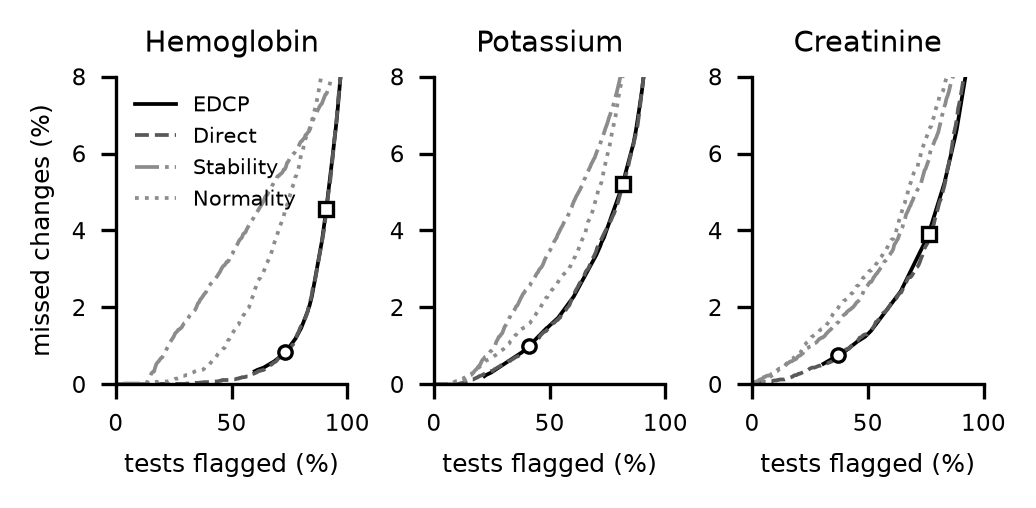
\includegraphics[width=\columnwidth]{fig_tradeoff}
\caption{Missed action changes versus share of tests flagged on the test patients as the threshold varies. Markers are the CRC operating points of EDCP at $\alpha=1\%$ (circle) and $5\%$ (square), selected on calibration patients.}\label{fig:tradeoff}
\end{figure}

A conventional probability cut-off of 0.5 offers no control over the miss rate. Applied to potassium, the normality classifier suppressed tests concealing 13.5\% action changes (as a share of all tests), and EDCP itself, without CRC, concealed 7.7\% for potassium and 9.9\% for creatinine. Fig.~\ref{fig:tradeoff} shows why the target matters: across the whole operating range, scores trained on the action label conceal far fewer changes than the proxy classifiers for the same number of suppressed tests.

\subsection{Certified reduction}
Under CRC, the mean miss rate across 100 re-partitions remained below $\alpha$ for every analyte and every level from 0.5\% to 5\%. At $\alpha=1\%$ the low-value tier comprised 73.8\% of hemoglobin, 41.3\% of potassium and 38.1\% of creatinine tests (Table~\ref{tab:perf}). The guarantee is in expectation, and individual partitions occasionally exceeded the target (95th percentile 0.92--1.16\% at $\alpha=1\%$). Platelets are degenerate, because action changes were rarer than $\alpha$ for $\alpha\ge2\%$. At the most stringent level, $\alpha=0.5\%$, only 1.8\% of creatinine tests could be certified. With CRC applied to every comparator at $\alpha=5\%$, B5 retained slightly more tests than EDCP (potassium: 82.0\% versus 76.2\%), while the rule B1 retained 26--30\%. LTT ($\beta=5\%$, $\delta=0.1$) flagged 89.1\%, 71.8\% and 64.2\% of hemoglobin, potassium and creatinine tests. The patient-level variant met its own criterion for all analytes and levels with a similar tier size (77.9\% and 41.6\% for hemoglobin and potassium at $\alpha=1\%$). Within sex and age strata, miss rates at $\alpha=1\%$ ranged from 0.65\% to 1.17\% on the single test partition, and Mondrian calibration did not narrow this range consistently.

% source: results\challenge2019/E4/temporal.csv, results\challenge2019/E7/table10_online.csv (order=temporal)
\begin{table}[t]\centering\footnotesize
\caption{Transfer to an unseen hospital (models and calibration from hospital A, test stream from hospital B). Cells: missed action changes (\%) / tests avoided (\%). Online cells average five audit seeds.}
\label{tab:external}\setlength{\tabcolsep}{2.5pt}
\begin{tabular}{llcccc}\toprule
$\alpha$ & Lab & Static & Recalib. 20\% & Online $p{=}0.2$ & Online $p{=}0.1$ \\ \midrule
\multirow{4}{*}{1\%} & Hemoglobin & 1.62 / 61 & 0.67 / 51 & 1.03 / 44 & 1.06 / 49 \\
 & Potassium & 0.85 / 28 & 0.91 / 30 & 0.88 / 23 & 0.87 / 25 \\
 & Creatinine & 0.61 / 29 & 0.60 / 29 & 0.72 / 26 & 0.68 / 28 \\
 & Platelets & 1.41 / 98 & 0.80 / 96 & 1.04 / 77 & 0.93 / 84 \\
\midrule
\multirow{4}{*}{5\%} & Hemoglobin & 16.83 / 97 & 4.98 / 74 & 4.99 / 59 & 5.04 / 66 \\
 & Potassium & 5.50 / 79 & 3.96 / 70 & 5.01 / 60 & 5.15 / 68 \\
 & Creatinine & 4.15 / 78 & 4.10 / 78 & 4.96 / 66 & 4.64 / 72 \\
 & Platelets & 2.38 / 100 & 2.39 / 100 & 2.14 / 80 & 1.96 / 89 \\
\bottomrule\end{tabular}\end{table}


\subsection{Transfer to an unseen hospital}
Table~\ref{tab:external} summarizes the transfer from hospital A to hospital B. For potassium, creatinine and platelets the static threshold remained near its nominal level, whereas for hemoglobin it did not: 16.8\% of tests at hospital B were concealed action changes at a nominal 5\%, and 1.62\% at 1\%. Recalibration on 20\% of hospital B patients corrected the deviation but presupposes a labelled sample from the new site before deployment. The audited update requires no such sample. Auditing one flagged test in five reduced the hemoglobin miss rate to 4.99\% while 59\% of tests were still avoided (Fig.~\ref{fig:online}); auditing one in ten gave 5.04\% and 66\%. For this stream, Proposition~2 limits the estimated miss rate to 6.9\%. The guarantee is cumulative rather than windowed, and over the worst fifth of the stream the miss rate reached 5.7\%.

\begin{figure}[t]\centering
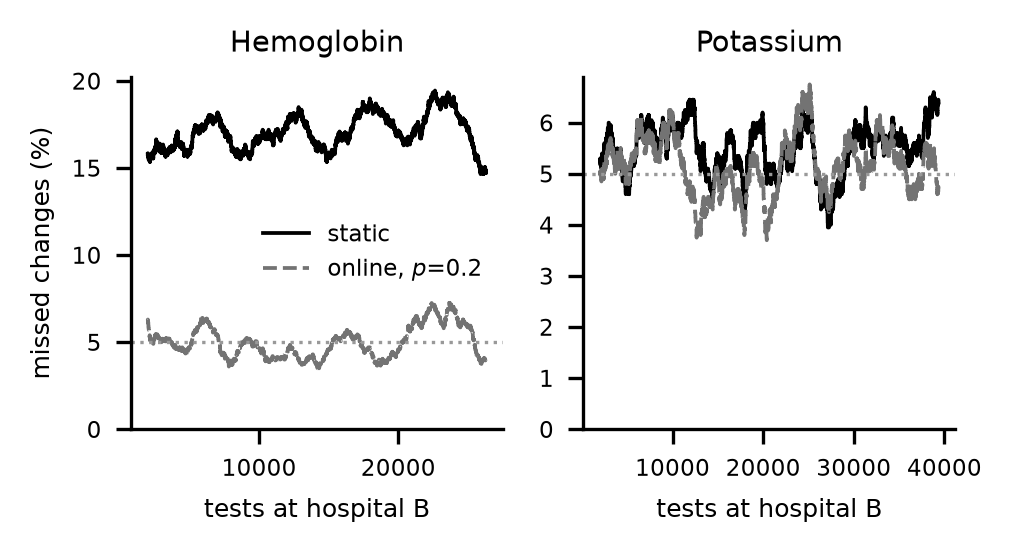
\includegraphics[width=\columnwidth]{fig_online}
\caption{Missed action changes at hospital B over a rolling window of 2,000 tests ($\alpha=5\%$, dotted). The static threshold was certified at hospital A; the online threshold audits 20\% of flagged tests.}\label{fig:online}
\end{figure}

% source: results\challenge2019/E7/table9_panel.csv
\begin{table}[t]\centering\footnotesize
\caption{Tube-level decisions. Cells: draws with a missed action change (\%) / draws avoided (\%), mean of 100 re-splits.}
\label{tab:panel}\setlength{\tabcolsep}{2.5pt}
\begin{tabular}{lcccc}\toprule
Draw & $\alpha$ & Per-lab at $\alpha$ & Bonferroni & Panel CRC \\ \midrule
CBC (Hgb + Plt) & 1\% & 1.20 / 71 & 0.51 / 61 & 0.79 / 69 \\
CBC (Hgb + Plt) & 5\% & 5.68 / 90 & 3.36 / 84 & 4.66 / 88 \\
BMP (K + Creat) & 1\% & 0.48 / 8 & 0.01 / 0 & 0.94 / 13 \\
BMP (K + Creat) & 5\% & 5.82 / 50 & 1.96 / 24 & 4.89 / 45 \\
\bottomrule\end{tabular}\end{table}


\subsection{Draw-level decisions}
Combining analyte-level certificates violated the draw-level target (Table~\ref{tab:panel}): 5.68\% for the CBC and 5.82\% for the chemistry draw at $\alpha=5\%$, and 1.20\% for the CBC at $\alpha=1\%$. Bonferroni correction was valid but conservative, avoiding only 24\% of chemistry draws at $\alpha=5\%$. Draw-level CRC met the target while avoiding 45\% of chemistry and 88\% of CBC draws at the same level. The eICU cohort reproduced the pattern (chemistry draw at $\alpha=5\%$: 6.46\% analyte-level versus 4.71\% draw-level).

\subsection{Explanations and ablations}
The ratio $\rho$ was strongly associated with EDCP (Spearman $-0.85$, $-0.95$ and $-0.93$ for hemoglobin, potassium and creatinine; $-0.49$ for platelets). Replacing the most influential feature of a test with a background value changed EDCP by 0.064, 0.102, 0.061 and 0.026 on average, compared with 0.001--0.007 for a randomly chosen feature (Wilcoxon $p<0.001$ for each analyte), and SHAP attributions summed to the model output within $3.5\times10^{-6}$. A representative output for potassium reads: ``Low value (certified at $\alpha=1\%$); predicted 4.3~mEq/L (80\% range 4.0--4.8), 0.80~mEq/L inside the current range; P(action change)~$\approx$~0.02.'' Removing the companion-analyte features had the largest effect, shrinking the tier at $\alpha=1\%$ from 73.8\% to 68.8\%, 41.3\% to 33.8\% and 38.1\% to 33.9\% for hemoglobin, potassium and creatinine. Omitting isotonic calibration preserved validity and slightly enlarged the tier.

\section{Discussion}
Three observations emerge. First, the target matters more than the learner: proxy labels overlook most potassium decisions, whereas two quite different models trained on the action label behave almost identically. Second, a certificate obtained at one hospital may not survive at another, and for hemoglobin the deviation was large despite the clinical similarity of the two sites. A model deployed with a fixed threshold would have appeared safe during validation yet been unsafe in use; the audited update corrected this at the expense of performing a small share of flagged tests, which doubles as continuous post-deployment monitoring. Third, the operative unit is the tube. Analyte-level certificates are convenient to report but do not describe the decision actually taken at the bedside.

Several limitations apply. The primary cohort is restricted to intensive care, is recorded at hourly resolution and lacks ethnicity, insurance and admission details, so subgroup analysis was confined to sex and age. Only ordered tests are observed; a test may have been requested precisely because a change was anticipated, and interventions between draws influence the next value. The action maps are simplified and ignore context such as active bleeding or cardiac disease. The analysis values one test at a time and ignores the option value of later tests. Finally, all guarantees are marginal and do not bound the miss rate for an individual patient.

\section{Conclusion}
CertiVOI evaluates each repeat test by the probability that its result alters the clinical action, and converts that probability into a tier with an explicit bound on concealed action changes. Certifying complete draws and adapting the threshold from audited results kept the bound intact in settings where a static analyte-level threshold failed. Future work will incorporate clinician-elicited utilities in place of 0--1 regret, validation on general wards, and a prospective audit study.

\section*{Acknowledgment}
The authors thank the PhysioNet team and the contributors to the Challenge 2019 and eICU databases for making the data openly available.

\bibliographystyle{IEEEtran}
\bibliography{refs}

\end{document}
